% unamblify -- Copyright (c) 2026 Rob Ludwick.
% SPDX-License-Identifier: AGPL-3.0-only
%
% Build: make          (tectonic)
%        make ENGINE=pdflatex
%
% Font: newtx (Times-like serif with matching maths). If newtx is not
% installed, comment the two \usepackage lines below and uncomment
% \usepackage{lmodern}; nothing else depends on the choice.
%
% Figures: spectrogram_comparison.pdf and the DVstick photo beside this
% source; the two model diagrams are TikZ, inline below.
\documentclass[10pt,twocolumn,a4paper]{article}

\usepackage[T1]{fontenc}
\usepackage[utf8]{inputenc}
\usepackage{newtxtext}
\usepackage{newtxmath}
% \usepackage{lmodern}   % fallback if newtx is unavailable
\usepackage[margin=19mm,columnsep=6mm]{geometry}
\usepackage{microtype}
\usepackage{booktabs}
\usepackage{array}
\usepackage{multirow}
\usepackage{amsmath}
\usepackage{siunitx}
\usepackage{graphicx}
\usepackage{tikz}
\usepackage{pgfplots}
\usepackage[font=small,labelfont=bf]{caption}
\usepackage[hidelinks]{hyperref}

\usetikzlibrary{arrows.meta,positioning,fit}
\pgfplotsset{compat=1.18}
\sisetup{group-separator={\,},group-minimum-digits=4,detect-all}

\setlength{\parskip}{0pt}
\setlength{\tabcolsep}{4pt}
\renewcommand{\arraystretch}{1.12}

% Shared style for the result curves.
\pgfplotsset{
  resultaxis/.style={
    width=0.92\columnwidth, height=46mm,
    xlabel={training step},
    scaled x ticks=false,
    xtick={0,10000,20000,30000,40000},
    xticklabels={0,10k,20k,30k,40k},
    xticklabel style={font=\scriptsize},
    yticklabel style={font=\scriptsize},
    label style={font=\scriptsize},
    legend style={font=\scriptsize, draw=none, fill=none},
    grid=both,
    major grid style={line width=0.2pt, draw=gray!25},
    minor grid style={draw=none},
    unbounded coords=discard, filter discard warning=false,
  }
}

% Reference values for the improvement chart: measurements of the
% unprocessed codec output and of clean speech, not of any training run.
\newcommand{\refcodeclsd}{19.2}      % raw AMBE decode vs clean, 0-4 kHz
\newcommand{\refcodechnr}{4.1}       % codec eval/hnr_abs, per-harmonic scale
\newcommand{\refcodecplos}{12.8}     % codec burst attenuation, dB
\newcommand{\refcleanmos}{4.05}      % UTMOS22, clean studio speech
\newcommand{\refcodecmos}{1.78}      % UTMOS22, codec decode
\newcommand{\refprevmos}{2.08}       % UTMOS22, first noise-head model
\newcommand{\hnrfloor}{0.75}         % hnr_abs measurement floor
% The corrected numbers of 25 September (experiment log row 38): the
% same judge, on the captured decode itself rather than a 16 kHz
% rendering of it, no synthetic tail.
\newcommand{\refcleanmosF}{4.14}     % UTMOS22, clean, faithful eval clips
\newcommand{\refcodecmosF}{2.22}     % UTMOS22, codec decode,
% faithful eval clips
\newcommand{\refpipemos}{3.57}       % UTMOS22, restorer + synthesizer

\title{\vspace{-8mm}\textbf{unamblify}: a real-time neural post-filter for\\
AMBE and Codec~2 digital voice}
\author{Rob Ludwick, AJ7HR\\[1ex]\normalsize
\url{https://rcludwick.github.io/unamblify}}
\date{25 September 2026}

% Let the two model diagrams and the spectrograms share one page.
\setcounter{dbltopnumber}{2}
\renewcommand{\dbltopfraction}{0.95}
\renewcommand{\dblfloatpagefraction}{0.8}

\begin{document}
\maketitle

\begin{abstract}
  \noindent
  Digital voice on amateur radio inherently operates at a low
  bitrate. Voice coders transmit a minimal set of parameters that
  describe speech, from which the receiver reconstructs the voice. As
  a result, current digital voice transmissions can be challenging to
  comprehend without prior listener acclimatization.

  At \SI{2400}{bit/s}, the AMBE family \cite{griffin1988mbe,hardwick1988mbe}
  discards phase information, inter-harmonic content, frequencies
  above \SI{3.7}{kHz}, and temporal structure finer than \SI{20}{ms}.

  \emph{unamblify} is a neural post-filter designed to operate after
  the decoder, inferring and restoring these missing components. The
  model is trained on paired recordings of clean speech and its
  corresponding degraded output from a vocoder. The dataset includes
  encodings from a hardware AMBE-3000R chip for D-STAR and YSF/DMR,
  and the \texttt{codec2} crate \cite{rowe2010codec2} for M17 modes.
  A Vocos-based \cite{siuzdak2024vocos} synthesizer was fine-tuned
  specifically for these digital voice modes. UTMOS22 \cite{saeki2022utmos} was used as
  the impartial judge.  The resulting model
  restores a significant portion of the information discarded during
  encoding. The primary goal of this project is to improve the
  intelligibility and naturalness of digital voice modes, thereby
  reducing the cognitive load required to understand transmissions.

\end{abstract}

\section{Introduction}
\label{sec:intro}

Digital voice modes on amateur radio use a vocoder. A vocoder does not
send the sound of your voice. Many times a second it measures a few
things about it:
\begin{itemize}\itemsep1pt
  \item the pitch,
  \item how loud each part of the frequency range is,
  \item whether each part is buzzing (voiced) or hissing (unvoiced).
\end{itemize}
The receiver reconstructs a new voice from
these parameters.

This is how complex speech waveforms can compress into a few thousand bits per second.
It is also why digital voice codecs can sound muffled and robotic.
The listener hears a reconstructed voice with clarity removed for efficiency.

\emph{unamblify} runs after the receiver's decoder. It uses two neural
networks. The first, the \emph{restorer}, reads the decoded audio and
predicts the spectrogram of the original speech. Here a spectrogram is
the energy in each of 100 frequency bands, about a hundred times a
second. The second network, the \emph{synthesizer}, turns that
spectrogram into audio.

The synthesizer is Vocos \cite{siuzdak2024vocos} fine-tuned on ham radio
codec audio.  Vocos itself was trained on
hundreds of hours of recorded speech and the spectrograms of that speech for AI voice synthesis.

The \emph{discriminator} is a third network, used only in training.  It
tries to distinguish the synthesizer's output from real recordings. The synthesizer was
rewarded when it fooled the discriminator.

The key understanding is that Vocos can only render the spectrogram it is given.
It cannot add detail that is missing. Given the blurred spectrogram of
a codec, it produces a blurred voice. That is why the restorer is used in front of
the synthesizer.

\subsection{What the codec throws away}

\begin{table}[t]
  \centering\footnotesize
  \setlength{\tabcolsep}{2pt}
  \caption{Vocoder bit rates on the air.}
  \label{tab:rates}
  \begin{tabular}{@{}llrrr@{}}
    \toprule
    Mode & Vocoder & Voice (bit/s) &  Total (bit/s) \\
    \midrule
    D-STAR            & AMBE          & 2400 & 3600 \\
    DMR               & AMBE+2        & 2450 & 3600 \\
    YSF (Narrow)      & AMBE+2        & 2450 & 3600 \\
    NXDN (Narrow)     & AMBE+2        & 2450 & 3600 \\
    M17 voice         & Codec~2 3200  & 3200 & 3200 \\
    M17 voice + data  & Codec~2 1600  & 1600 & 1600 \\
    \bottomrule
  \end{tabular}
\end{table}

Table~\ref{tab:rates} lists the bit rate of each mode.

AMBE does not try to keep the whole voice. It is based on the
multi-band excitation model. Each \SI{20}{ms} frame carries:
\begin{itemize}\itemsep1pt
  \item the pitch (7~bits),
  \item one voiced or unvoiced decision per band of about
    \SI{500}{Hz},
  \item the spectral envelope, sampled once per harmonic (57~bits, or
    37 in AMBE+2).
\end{itemize}

Five things are discarded:

\begin{enumerate}\itemsep2pt
  \item Phase. The receiver has to make it up.
  \item Everything between the harmonics.
  \item Everything above \SI{3.7}{kHz}.
  \item Fine voicing detail. Each band gets one voiced or unvoiced bit
    per \SI{20}{ms}. Breathy, mixed, and changing sounds are forced to
    one side.
  \item Timing inside the frame. Every value is an average over
    \SI{20}{ms}, so the start of a consonant is smeared.
\end{enumerate}

Together these cause the familiar digital-voice sound. The author
noticed that non-native speakers on AMBE+2 narrow usually took more effort to
understand than on a clean recording. This project aims to reduce the cognitive
effort by restoring what the codec leaves out.

\section{Goals}
\label{sec:goals}

\textbf{1. Natural narrowband.} Remove the buzz and the
robotic sound, and restore the texture of unvoiced sounds and transients,
at the vocoder's \SI{8}{kHz} rate.
The reference for ``good'' is a clean SSB voice without audible digital distortions.

\textbf{2. Bandwidth extension.} Output at \SI{16}{kHz} with
plausible \SIrange{4}{8}{kHz} content. The reference here is an AM broadcast
voice.

\textbf{3. Real time in Rust.} \SI{20}{ms} frames,
streaming, with a low and fixed added latency, and small enough to run
alongside the rest of a client's audio pipeline.

\textbf{4. Reproducible.} Which corpora were used, how they were
fetched, how they were pushed through the hardware, and how the model
was trained are all scripted and documented.

\section{What was learned, in short}
\label{sec:learned}

This section summarizes the key findings, which are detailed in the
remainder of the paper.

For the first attempt a post-filter was implemented.
Because the codec discards information, a post-filter can only reshape the remaining signal.
The initial model (figure~\ref{fig:arch1}) functioned as a filter.
The network observed the decoder's output and adjusted it 100 times per second.
It was computationally lightweight, running in a tenth of a millisecond per frame.

Unfortunately, its performance plateaued. Adding more data without increasing the
step count degraded performance.

The second model (figure~\ref{fig:arch2}) generates a new spectrum
before synthesizing the voice. It consists of two interfaced networks. A \emph{restorer}
processes the codec output and predicts the original wideband
spectrum, generating 100 values every \SI{10}{ms} with an \SI{85}{ms}
lookahead. The \emph{synthesizer} then converts this spectrum
into audio.

Data quality was more impactful than network architecture. Common
Voice accounts for 90 percent of the samples, but these volunteer
recordings vary in microphone and room dynamics. Training the
restorer on the 10 percent of studio-recorded data yielded the most
significant improvements.

Table~\ref{tab:learned} summarizes the current performance. In a
blind listening test with 16 held-out speakers across four
level-matched systems, the regenerated speech showed notable
improvement, often sounding very close to the original recordings.
Furthermore, UTMOS22~\cite{saeki2022utmos} evaluations indicated
a measurable improvement over the raw codec output.

\begin{table}[t]
  \centering\small
  \caption{80 evaluation clips were judged by UTMOS22, and 64 clips each from
    DMR and D-STAR were blindly judged by the author.}
  \label{tab:learned}
  \begin{tabular}{@{}lccc@{}}
    \toprule
    & UTMOS22 & \multicolumn{2}{c}{blind listening test} \\
    & (1--5) & D-STAR & YSF/DMR \\
    \midrule
    original recording     & \refcleanmosF{} & 4.9$^{\ddagger}$ & 5.0 \\
    raw codec              & \refcodecmosF{} & 1.6 & 1.9 \\
    filter model (first)   & 2.1$^{\dagger}$ & 2.6 & 2.6 \\
    restorer + synthesizer & \textbf{\refpipemos{}} & \textbf{4.6} &
    \textbf{4.6} \\
    \bottomrule
  \end{tabular}

  \smallskip
  {\scriptsize $^{\dagger}$Measured on an earlier clip set, where the
    codec scored 1.79 and the recording 4.10.
    $^{\ddagger}$Different
    audio samples were judged with D-STAR and YSF/DMR. Not all
    original samples were of high quality.
  }
\end{table}

Figure~\ref{fig:spectrogram_comparison} shows the second model on one
held-out utterance. The AMBE decoder discards all speech content above
\SI{3.7}{kHz} and flattens the detail between harmonics. The restorer
and synthesizer rebuild the upper band and the vocal continuity.

\subsection{What needs improvement}
Stop consonants are \SIrange{5}{8}{dB}
quieter than the recording, with the codec's smear halved; the filter
had made them worse than the codec. The ``s'' is
\SI{4.5}{dB} soft.

\section{Generating the training set}
\label{sec:data}

Producing the training pairs at scale is most of the effort in the
project.
While Codec~2 can be parallelized to deliver quick results,
the AMBE chip runs closer to real time, so the corpus is bounded by weeks of wall-clock
time and not by disk or compute.

\begin{figure}[htb]
  \centering
  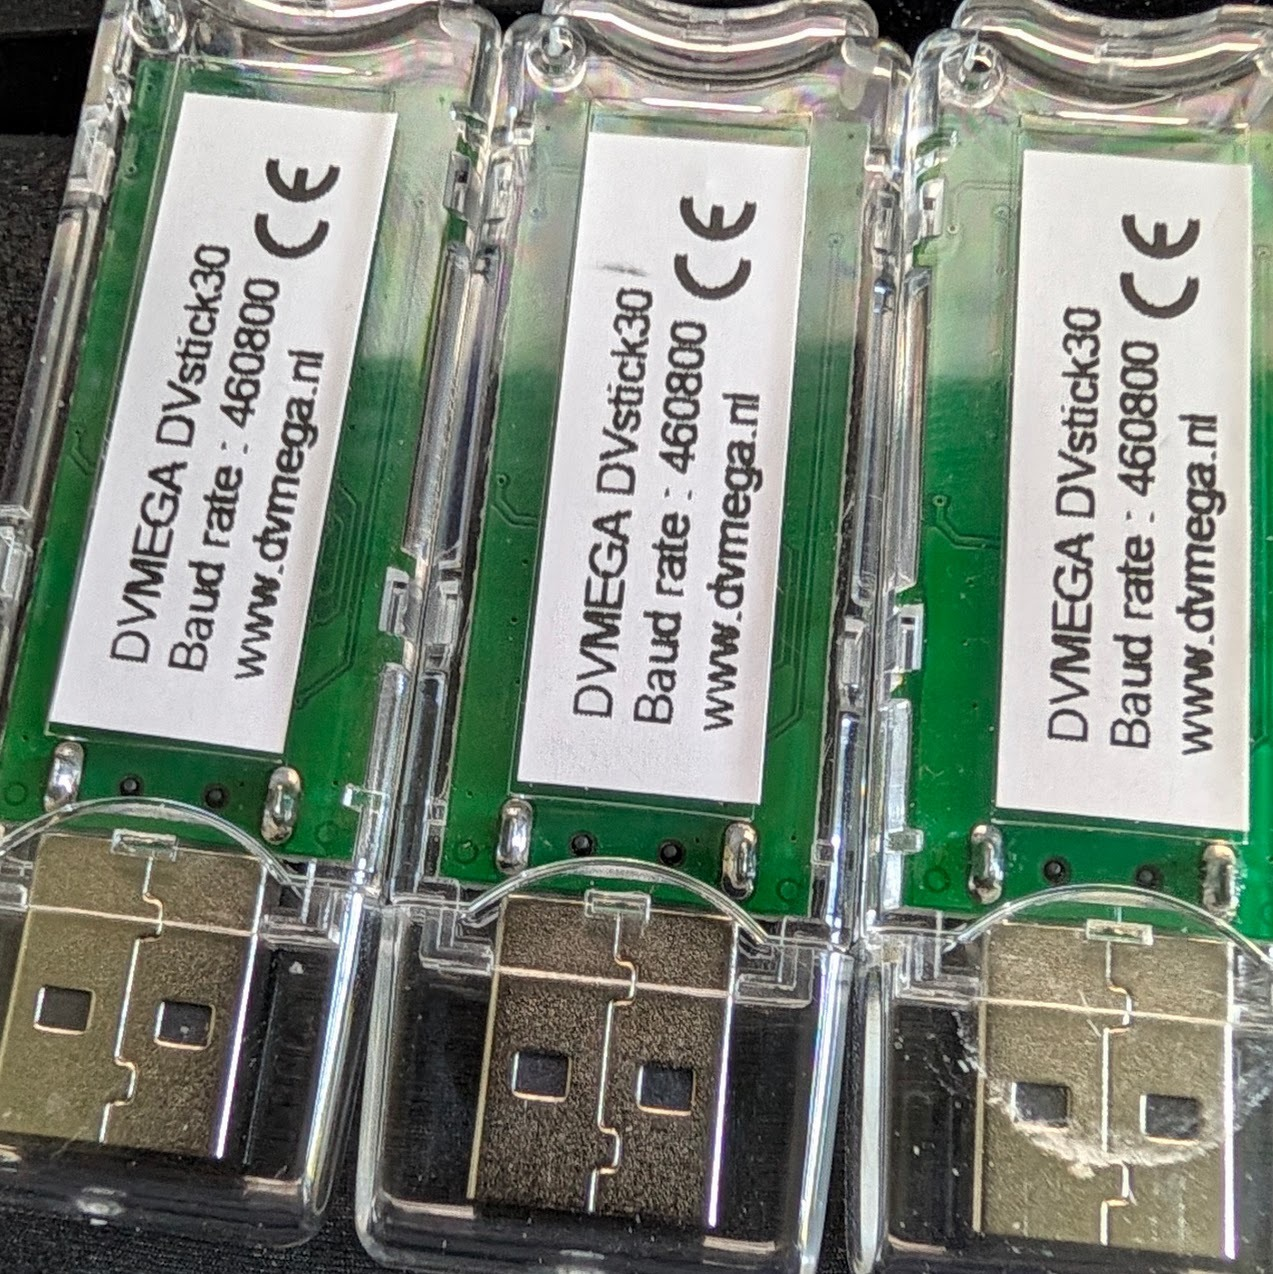
\includegraphics[width=0.6\columnwidth]{PXL_20260914_234231998.MACRO_FOCUS.jpg}
  \caption{The three DVMEGA DVstick~30s that run the AMBE captures. Each
    holds a DVSI AMBE-3000R chip behind a USB serial link at
    \num{460800} baud, and each runs one capture worker.}
  \label{fig:dvsticks}
\end{figure}

\tikzset{
  blk/.style={draw, rounded corners=1.5pt, align=center, font=\scriptsize,
    inner sep=2.5pt, minimum height=6mm},
  io/.style={blk, fill=gray!12},
  head/.style={blk, fill=blue!6},
  ar/.style={-{Latex[length=1.6mm]}, thin},
  grp/.style={draw, dashed, gray, rounded corners=3pt, inner sep=2.5mm},
}

\begin{figure*}[t]
  \centering
  \begin{minipage}[b]{0.48\textwidth}
  \centering
  \begin{tikzpicture}[node distance=3.2mm and 2.5mm]
    \node[io] (in) {decoder output, \SI{8}{kHz}};
    \node[blk, below=of in] (fc) {frame conv\\\SI{20}{ms} window, \SI{10}{ms} hop};
    \node[blk, below=of fc] (cc) {context conv\\\SI{80}{ms} back, lookahead ahead};
    \node[blk, right=3mm of cc, fill=gray!5] (mode) {mode\\tag};
    \node[blk, below=of cc] (gru) {2-layer GRU, 256 wide};
    \node[head, below=5mm of gru] (comb) {comb filter\\24 pitch lags};
    \node[head, left=of comb] (fir) {FIR filter\\16 taps};
    \node[head, right=of comb] (noise) {noise\\head};
    \node[blk, below=of comb] (sum) {filter the received audio,\\add the noise};
    \node[blk, below=of sum] (up) {half-band upsampler, $\times 2$};
    \node[blk, below=of up] (bwe) {bandwidth extension};
    \node[io, below=of bwe] (out) {output, \SI{16}{kHz}};
    \draw[ar] (in) -- (fc); \draw[ar] (fc) -- (cc); \draw[ar] (cc) -- (gru);
    \draw[ar] (mode) |- (gru);
    \draw[ar] (gru) -- (comb); \draw[ar] (gru.south) -- (fir.north); \draw[ar] (gru.south) -- (noise.north);
    \draw[ar] (fir) -- (sum); \draw[ar] (comb) -- (sum); \draw[ar] (noise) -- (sum);
    \draw[ar] (sum) -- (up); \draw[ar] (up) -- (bwe); \draw[ar] (bwe) -- (out);
    \draw[ar, dashed] (in.west) -- ([xshift=-6mm]in.west -| fir.west) |- (sum.west);
    \draw[ar] (gru.east) -- ([xshift=3mm]gru.east -| noise.east) |- (bwe.east);
    \node[grp, fit=(fc)(cc)(mode)(fir)(noise)(sum)(up)(bwe)] (fgrp) {};
    \node[font=\scriptsize, gray, anchor=north, rotate=90] at (fgrp.east) {filter, \num{2.1}M parameters, \SI{8.5}{MB} at 32-bit};
  \end{tikzpicture}
  \caption{The first model, an adaptive filter in the manner of LACE and NoLACE \cite{buthe2024nolace}: \num{2124326} parameters, \SI{8.5}{MB} of 32-bit weights.
    Every \SI{10}{ms} the GRU sets the taps of a short FIR filter, the
    mix of a pitch comb and, in later runs, the level of a noise source. They are applied
    to the received audio itself (dashed). A fixed upsampler and a small
    bandwidth-extension head take the result to \SI{16}{kHz}.}
  \label{fig:arch1}
  \end{minipage}\hfill
  \begin{minipage}[b]{0.48\textwidth}
  \centering
  \begin{tikzpicture}[node distance=3.2mm and 2.5mm]
    \node[io] (in) {decoder output, \SI{8}{kHz}};
    \node[blk, below=of in] (stft) {resample to \SI{24}{kHz}, STFT};
    \node[blk, below=of stft] (low) {low-band\\log spectrum\\171 bins};
    \node[blk, left=of low, fill=gray!5] (mode) {mode\\tag};
    \node[blk, right=of low] (mel) {mel spectrum\\of the decoder\\output, 100 bands};
    \node[blk, below=of low, minimum width=44mm] (cin) {input conv, 2 frames ahead};
    \node[blk, below=of cin] (blocks) {6 conv blocks\\first two look 3 frames ahead};
    \node[blk, below=of blocks] (gru) {GRU, 384 wide};
    \node[blk, below=of gru] (lin) {linear, 100 bands};
    \node[blk, below=of lin] (plus) {apply the correction:\\a gain per band, every \SI{10.7}{ms}};
    \node[io, below=of plus] (pmel) {predicted clean mel\\100 bands, \SI{10.7}{ms}};
    \node[head, below=5mm of pmel] (voc) {Vocos synthesizer\\convolutions, inverse STFT};
    \node[io, below=of voc] (out) {output, \SI{24}{kHz}};
    \draw[ar] (in) -- (stft); \draw[ar] (stft) -- (low); \draw[ar] (stft.south) -- (mel.north);
    \draw[ar] (low) -- (cin); \draw[ar] (mode) -- (mode |- cin.north); \draw[ar] (mel) -- (mel |- cin.north);
    \draw[ar] (cin) -- (blocks); \draw[ar] (blocks) -- (gru); \draw[ar] (gru) -- (lin);
    \draw[ar] (lin) -- (plus); \draw[ar] (plus) -- (pmel); \draw[ar] (pmel) -- (voc); \draw[ar] (voc) -- (out);
    \draw[ar, dashed] (mel.east) -- ++(2mm,0) |- (plus.east);
    \coordinate (melpad) at ([xshift=4mm]mel.east);
    \node[grp, fit=(mode)(mel)(cin)(blocks)(gru)(lin)(plus)(melpad)] (rgrp) {};
    \node[font=\scriptsize, gray, anchor=south west, rotate=90] at (rgrp.south west) {restorer, \num{6.8}M};
    \node[grp, fit=(voc)] (sgrp) {};
    \node[font=\scriptsize, gray, anchor=west] at (sgrp.east) {synthesizer, \num{13.5}M};
  \end{tikzpicture}
  \caption{The second model, a restorer and a waveform synthesizer.
    The restorer predicts a correction to the mel spectrum of the
    decoder output, before any restoration (the dashed residual path) with \SI{85}{ms} of lookahead. Vocos,
    fine-tuned on the restorer's predictions, turns the corrected
    spectrum into \SI{24}{kHz} audio.}
  \label{fig:arch2}
  \end{minipage}
\end{figure*}



\begin{figure*}[t]
  \centering
  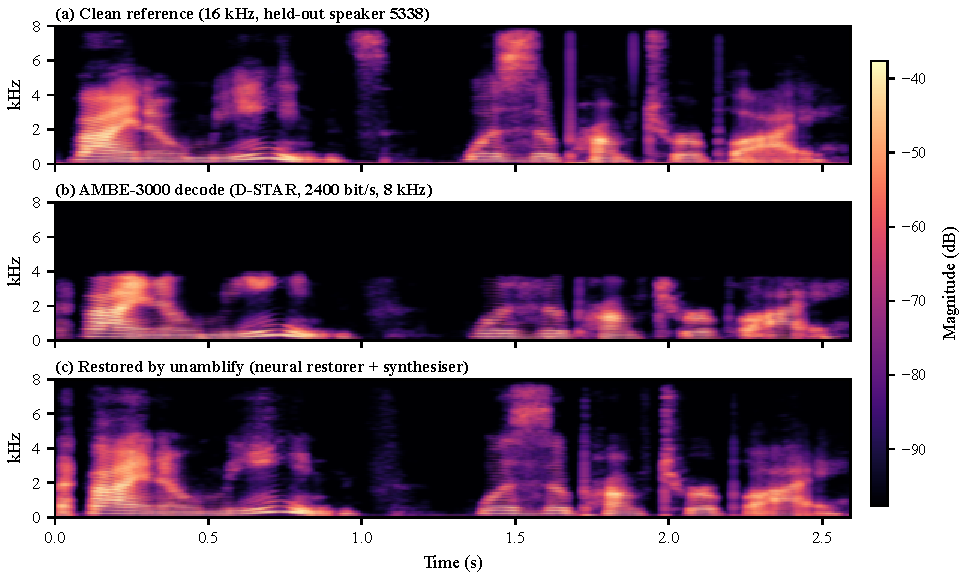
\includegraphics[width=0.98\textwidth]{spectrogram_comparison.pdf}
  \caption{Log-magnitude spectrograms for a held-out evaluation
    utterance (LibriTTS-R, speaker 5338).
    (a)~Clean \SI{16}{kHz} studio reference.
    (b)~AMBE-3000R hardware decode (D-STAR mode, \SI{2400}{bit/s},
    \SI{8}{kHz}), illustrating the hard cutoff at \SI{3.7}{kHz}.
    (c)~Restored audio from \emph{unamblify} (neural restorer plus
    synthesizer), showing reconstructed wideband harmonics up to
  \SI{8}{kHz}.}
  \label{fig:spectrogram_comparison}
\end{figure*}


\subsection{The codecs}
\label{sec:codecs}

Every training pair is clean speech beside the same speech after one
real codec. Table~\ref{tab:codecs} lists the codecs used. Each one
produces its own capture set, named as the harness names it.

\begin{table}[t]
  \centering\small
  \caption{The codecs behind the capture sets. Lag is the decoder's
  delay in samples at \SI{8}{kHz}, measured per set by cross-correlation.}
  \label{tab:codecs}
  \begin{tabular}{@{}lllr@{}}
    \toprule
    Set & Codec & Implementation & Lag \\
    \midrule
    \texttt{dstar}        & AMBE    & AMBE-3000R chip   & 326 \\
    \texttt{ysf-dmr}      & AMBE+2  & AMBE-3000R chip   & 381 \\
    \texttt{dstar+perens} & AMBE    & software (Perens) & 216 \\
    \texttt{codec2-3200}  & Codec~2 & \texttt{codec2} crate & 140 \\
    \texttt{codec2-1600}  & Codec~2 & \texttt{codec2} crate & 140 \\
    \bottomrule
  \end{tabular}
\end{table}

\textbf{D-STAR through the chip} (\texttt{dstar}). The AMBE-3000R is
DVSI's own implementation and the one real D-STAR radios contain, so
this set is the reference for the mode. The chip is set to the D-STAR
rate word: \SI{2400}{bit/s} of voice in \SI{20}{ms} frames.

\textbf{AMBE+2 through the chip} (\texttt{ysf-dmr}). The same chip at
the AMBE+2 half rate, \SI{2450}{bit/s}. System Fusion DN, DMR, and NXDN
all use this vocoder mode. YSF~DN and DMR carry the same 49 voice bits
per frame and differ only in framing and error correction, so one
capture serves both.

\textbf{Bruce Perens' D-STAR implementation} (\texttt{dstar+perens}).
The same prepared
audio re-encoded by a second, independent implementation of the D-STAR
vocoder: the floating-point AMBE path from Bruce Perens'
\texttt{hams\_open} \cite{perens2026hamsopen} (LGPL-3.0-or-later), vendored in the repository.
It produces the same bitstream format but not the chip's audio exactly.\footnote{Bruce Perens recently said it was around 97 percent accurate.}
This implementation also scores lower on predicted MOS (2.18 against the chip's 2.56).

\textbf{Codec~2 at 3200 and 1600 bit/s} (\texttt{codec2-3200},
\texttt{codec2-1600}). M17's two voice modes, through the
\texttt{codec2} Rust crate (version 0.3.1, a port of David Rowe's
reference). The 3200 mode uses \SI{20}{ms} frames and the 1600 mode
\SI{40}{ms}, both 64 bits per frame. Software capture is fast, so these
sets cover the whole prepared corpus (section~\ref{sec:data}).

\textbf{Lost frames} (\texttt{+drops}). A sibling of a set, not a new
codec. The stored channel frames of an existing capture have some
frames dropped and substituted, then only the decode is re-run. The
model sees what a receiver hears when frames go missing on the air.

\subsection{The corpus}

Table~\ref{tab:corpus} is what has been prepared and how much of it
has been through each codec.

\begin{table*}[t]
  \centering\small
  \caption{Prepared and captured utterances, 25 September 2026.}
  \label{tab:corpus}
  \begin{tabular}{@{}lrrrrrrr@{}}
    \toprule
    & \multicolumn{3}{c}{Prepared} & \multicolumn{4}{c}{Captured} \\
    \cmidrule(lr){2-4}\cmidrule(l){5-8}
    Corpus & Utterances & Hours & Speakers & D-STAR & D-STAR (Perens) & YSF/DMR & Codec~2 \\
    \midrule
    Common Voice (en) \cite{ardila2020commonvoice} & \num{1937661} & 2294.4 & \num{83816} &
    \num{309220} & \num{53987} & \num{148794} & \num{1937661} \\
    LibriTTS-R \cite{koizumi2023librittsr} & \num{347709}  &  566.5 & \num{2385}  &
    \num{152799} & \num{4182} & \num{152799} & \num{347709}  \\
    Hi-Fi TTS \cite{bakhturina2021hifitts} & \num{257288}  &  241.0 & 8           & 0
    & 0 & 0            & \num{257288}  \\
    VCTK 0.92 \cite{yamagishi2019vctk} & \num{44304}   &   32.0 & 110         &
    \num{44304}  & \num{1210} & \num{44304}  & \num{44304}   \\
    LJSpeech 1.1 \cite{ito2017ljspeech} & \num{13100}   &   23.9 & 1           &
    \num{13100}  & \num{381} & \num{13100}  & \num{13100}   \\
    VoiceBank-DEMAND \cite{valentini2017voicebank} & \num{12387}   &    9.4 & 30          &
    \num{12387}  & \num{330} & \num{12387}  & \num{12387}   \\
    Twins             & \num{42571}   &        &             &
    \num{42571}  & \num{42571} & \num{42571}  & \num{42571}   \\
    \midrule
    Total             & \num{2655020} & 3167.2 & \num{86350} &
    \num{574381} & \num{102661} & \num{413955} & \num{2655020} \\
    \bottomrule
  \end{tabular}
\end{table*}

\subsection{Preparation}

Preparation processes each source utterance through a series of steps:

\begin{enumerate}\itemsep2pt
  \item \textbf{Decode and resample}: Decode each source file (WAV,
    FLAC, or MP3) and resample to \SI{16}{kHz} with a band-limited
    sinc resampler. A 256-tap Blackman-Harris$^2$ windowed sinc
    (cutoff at 0.95 Nyquist) with group-delay compensation ensures
    sample-accurate phase and timing alignment.
  \item \textbf{Trim silence}: Strip leading and trailing silence
    below \SI{-45}{dBFS} while keeping a \SI{200}{ms} margin.
  \item \textbf{Normalize}: Scale active-speech RMS to \SI{-26}{dBFS}.
  \item \textbf{Filter duration}: Discard any utterance under one second.
  \item \textbf{Export aligned pairs}: Write two aligned files per
    utterance: a \SI{16}{kHz} target signal and an \SI{8}{kHz}
    decimated copy for the vocoder.
\end{enumerate}

The corpus is split into ``train'', ``dev'' and ``test'' groups by
speaker, guaranteeing no speaker appears in two splits.

\subsection{Augmentation}

We add noise to the clean speech and push it through a synthetic
overdriven transmit chain to create ``twin'' utterances.  These 
twins are then used as the input to the codec.  Bit losses before
the codec and audio distortions before and after the codec
are added.  This makes the model more effective for real-world
conditions.

\subsection{Shards}
\label{sec:shards}

The final stage joins the capture manifests with the prepared manifest
and packs fixed-length training examples into shards, which are flat
files the trainer can memory-map.

The filter model's largest set held \num{100000} utterances:
\num{40000} YSF/DMR, \num{30000} D-STAR, and \num{15000} each of
Codec~2 3200 and 1600. YSF/DMR got the largest share because it is
the mode the codec damages most. The restorer is trained on a set drawn
only from the studio corpora (LibriTTS-R, VCTK, LJSpeech,
VoiceBank-DEMAND and Hi-Fi TTS), with up to \num{500000} utterances
from each capture set.

\section{The two models}
\label{sec:results}

Two architectures have been tested. The first is a filter. It
reshapes the decoder's output and cannot add what the codec removed.
The second predicts the clean spectrum and synthesizes a new waveform
from it. Figures~\ref{fig:arch1} and~\ref{fig:arch2} show both, and
both are judged by predicted MOS.

Predicted MOS from UTMOS22 \cite{saeki2022utmos} is the objective judge. UTMOS22
is trained on human ratings and is not part of the training, so it cannot be
optimized against or gamed.

The filter architecture (figure~\ref{fig:arch1}) runs in a tenth of a millisecond
per frame on one CPU core. Its best predicted MOS was 2.12, against
\refcodecmos{} for the codec, at step \num{76000} of an \num{80000}-step run, and that
turned out to be its ceiling. A probe showed why. Each clip was
rebuilt from the filter's output below \SI{3.8}{kHz} and the clean
recording above it, and scored. It scored 2.72, against 2.76 for the
codec's own low band in the same mix. A filter can only reshape
what the codec kept.

The restorer and synthesizer (figure~\ref{fig:arch2}) score \refpipemos{} on MOS, against
\refcodecmosF{} for the codec and \refcleanmosF{} for the original
recordings, measured on the list of captured decodes of the held-out clips.

\section{Status and what comes next}
\label{sec:status}

The data harness was built to monitor preparation, capture in hardware,
and training through a web page.  The AMBE captures take the longest
time and will run for several weeks, whereas the Codec~2 modes have
been completed.  The harness is Rust and AGPL-3.0-only, and the filter
models also use Rust.

The \emph{restorer + synthesizer} model will need to be optimized for
less powerful CPUs. One target is LinHT, the M17 Project's open
handheld radio, built on an NXP i.MX~93 processor with two Cortex-A55
cores. It is not yet clear whether that is enough to run the current
model in real time.

Further work will be needed to distill the model for embedded CPUs with
even further restricted computation and memory requirements.

\section*{Biography}

% Author biography. Replace the placeholder line below.
Rob Ludwick, AJ7HR. \emph{[Rob has been a licensed amateur radio operator since November 2025,
when he received his Extra Class license.  He graduated from Iowa State University with 
a bachelor's degree in computer engineering. He currently works as a software engineer for what
vaguely appears to be a large financial institution of some kind or another.]}
Callsign page: \url{https://www.qrz.com/db/AJ7HR}.

\bibliographystyle{plain}
\bibliography{bibliography}

\end{document}
